\section*{Instruction Manual}

\subsection*{Minimal Instruction Set}

\begin{figure}[H]
	\begin{center}
		\begin{tikzpicture}
			\node[,inner sep=0] at (0,0) {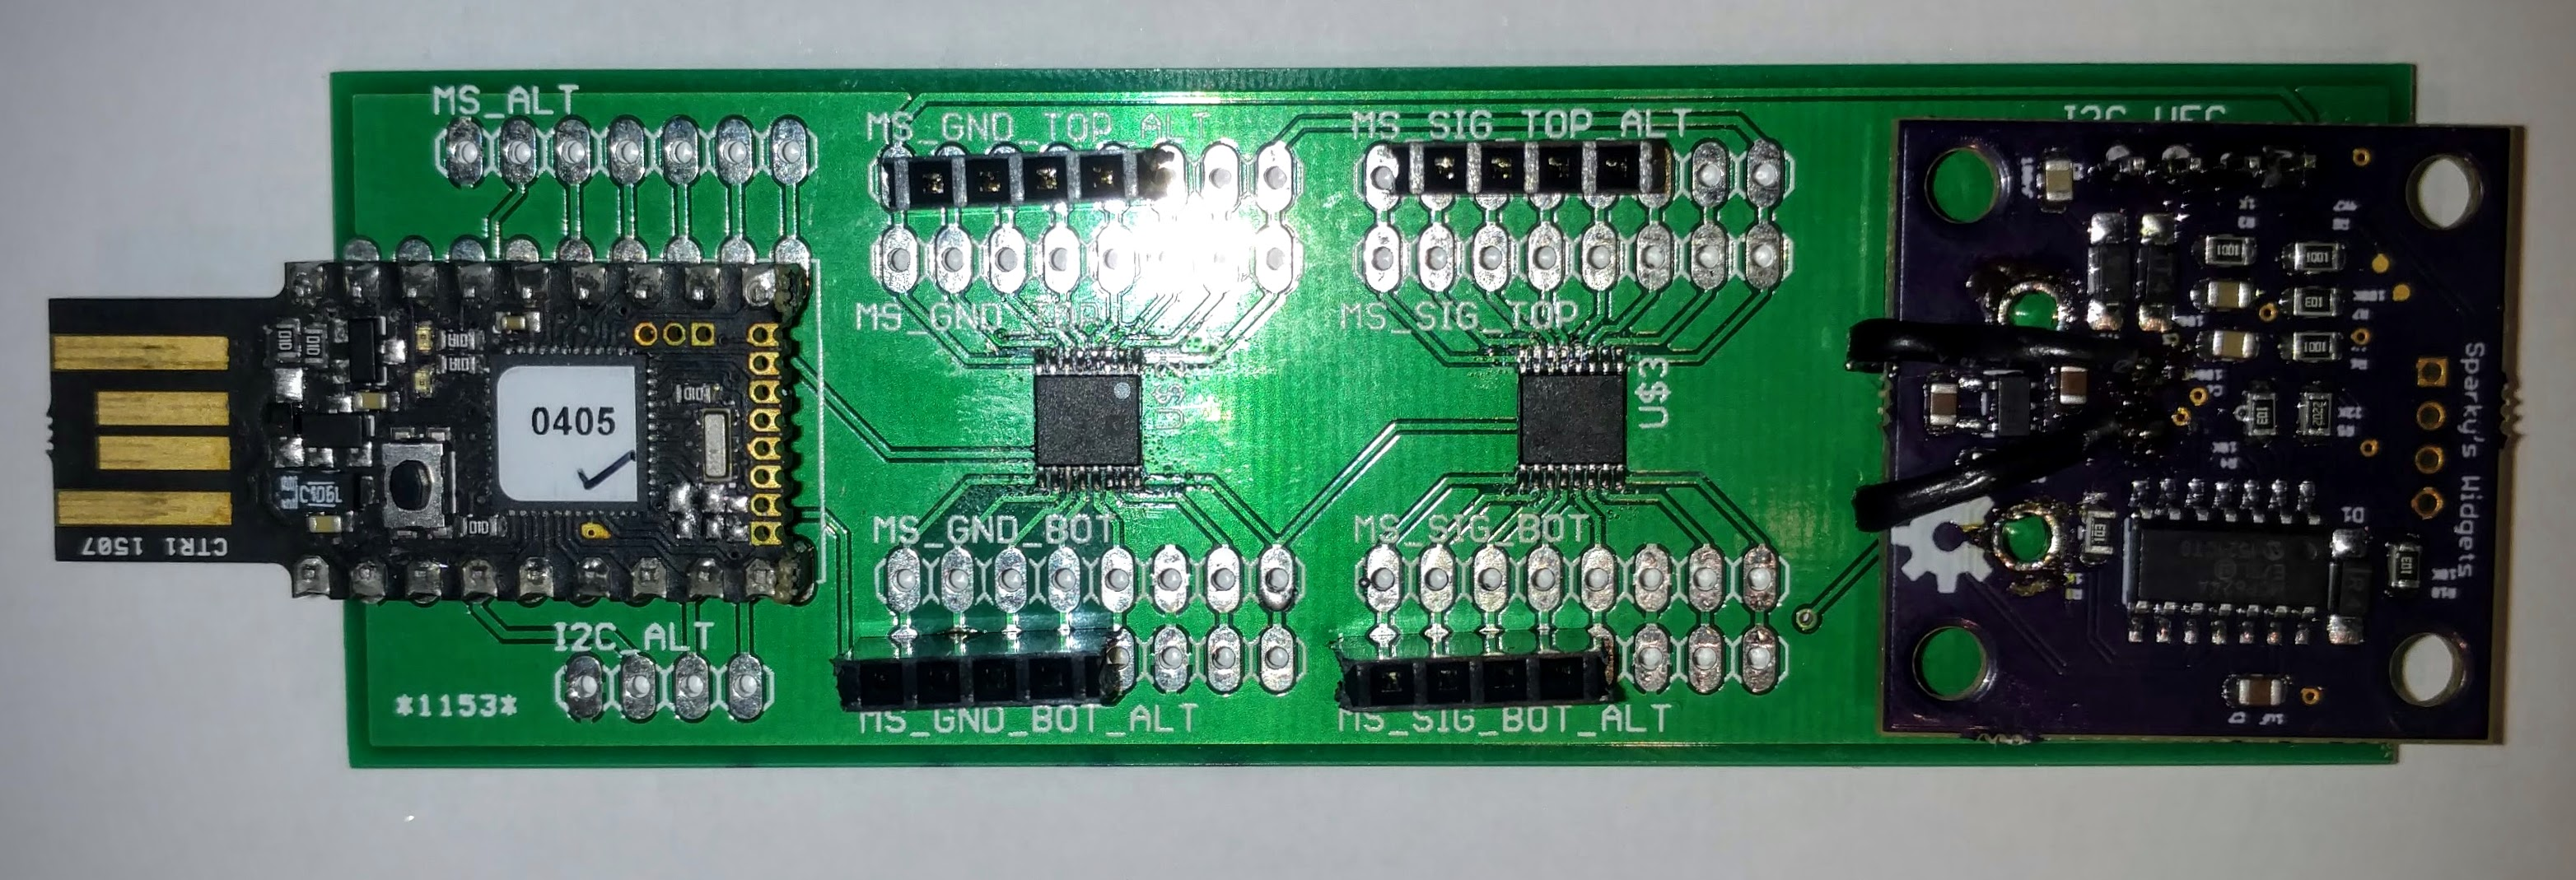
\includegraphics[width=0.5\textwidth]{images/cb.jpg}};
			\node[inner sep=0] at (0,-3) {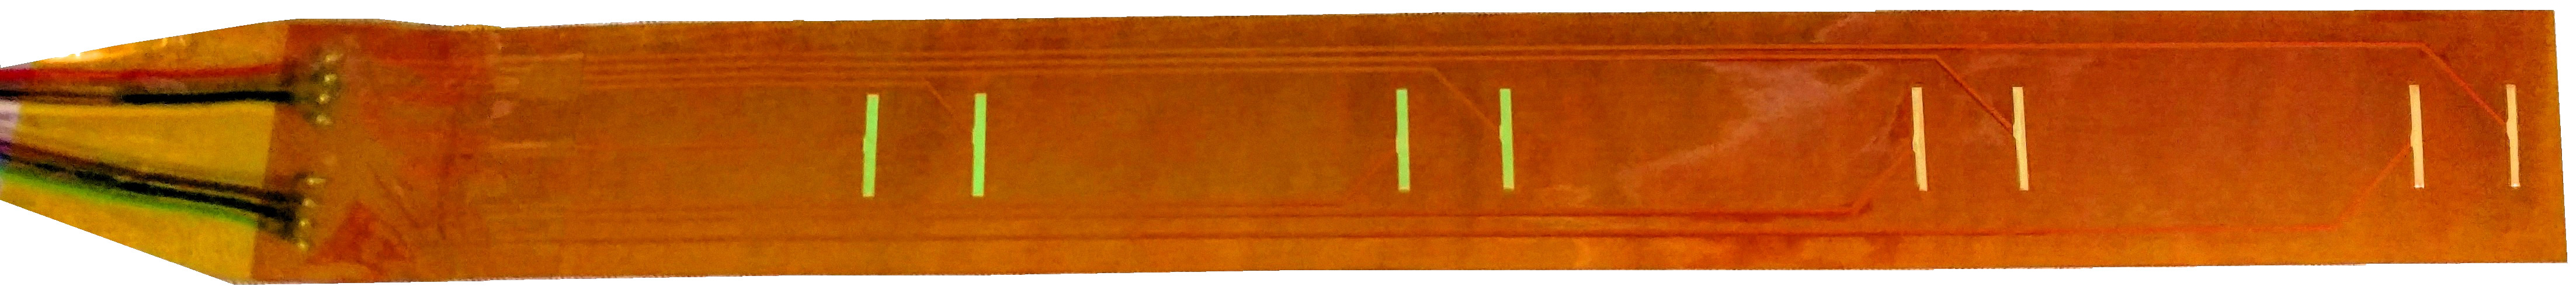
\includegraphics[width=\textwidth]{images/fpcbp.jpg}};
			
			\draw[red,ultra thick,rounded corners] (-4,-0.55) rectangle (-3.25,0.55);
			
			%\draw[red!50!yellow,ultra thick,rounded corners] (-1,-0.35) rectangle (-0.25,0.35);
			%\draw[red!50!yellow,ultra thick,rounded corners] (0.55,-0.35) rectangle (1.3,0.35);
			
			\draw[red!25!yellow,ultra thick,rounded corners] (-1.45,-1) rectangle (-0.3,-0.6);
			\draw[red!25!yellow,ultra thick,rounded corners] (0.3,-1.05) rectangle (1.3,-0.65);
			\draw[red!25!yellow,ultra thick,rounded corners] (-1.54,1.05) rectangle (-0.44,0.65);
			\draw[red!25!yellow,ultra thick,rounded corners] (0.15,1.05) rectangle (1.15,0.65);
			
			%\draw[blue,ultra thick,rounded corners] (1.8,-1.2) rectangle (4,1.2);
			\draw[blue!75!white,ultra thick,rounded corners] (-8,-4) rectangle (8,-2);
			%\draw[blue!50!white,ultra thick,rounded corners] (-2.75,-3.5) rectangle (-1.65,-2.5);
		\end{tikzpicture}
		\caption{USB connection (\drawline[red,ultra thick])\\sensor strip (\drawline[blue!75!white,ultra thick])\\connectors (\drawline[red!25!yellow,ultra thick])}
		\label{fig:isys}
	\end{center}
\end{figure}

\begin{itemize}
	\item[1] Use electrical tape to mount the sensor strips at desired points of measurement. Make sure not to cover the electrodes (golden parts).
	\item[2] Connect the cables of the sensor strip to the carrier board as shown in the picture:
	\begin{figure}[H]
	\begin{center}
		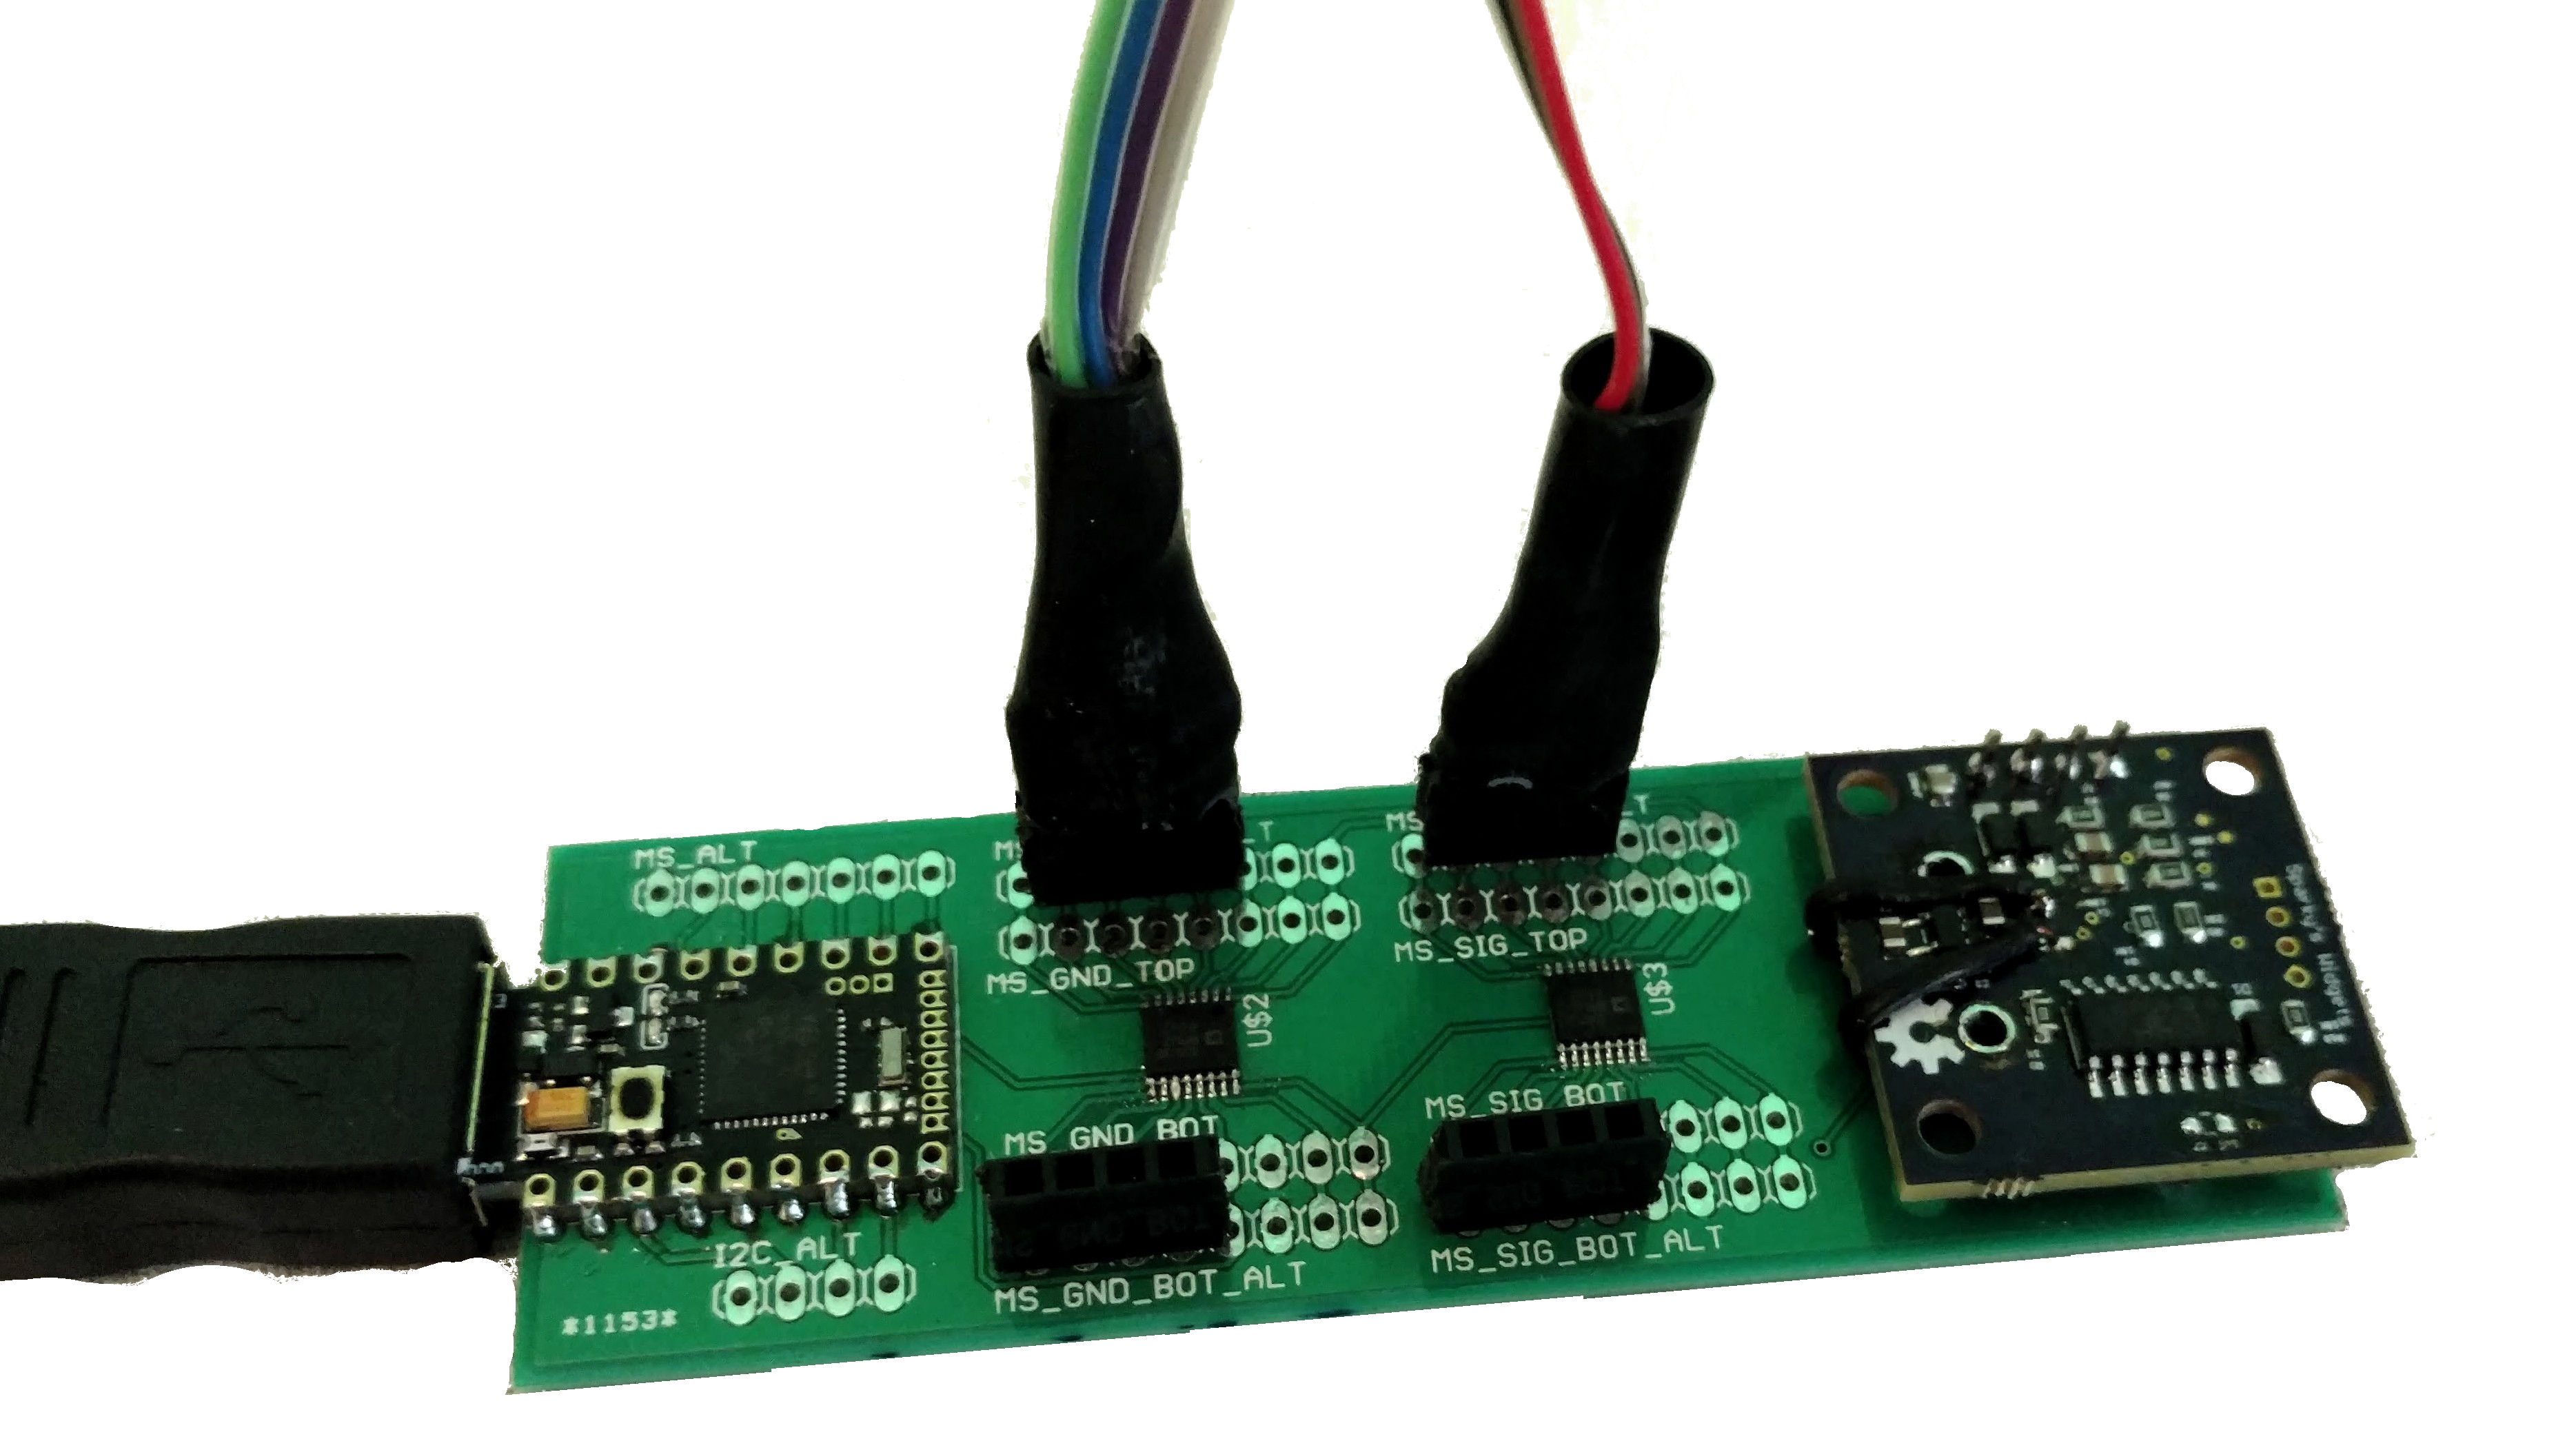
\includegraphics[width=0.5\textwidth]{images/conn.jpg}
		\caption{connectors}
		\label{fig:isys}
	\end{center}
\end{figure}
	\item[3] Connect the carrier board to the host PC with the USB cable. Note the orientation in the picture:
		\begin{figure}[H]
	\begin{center}
		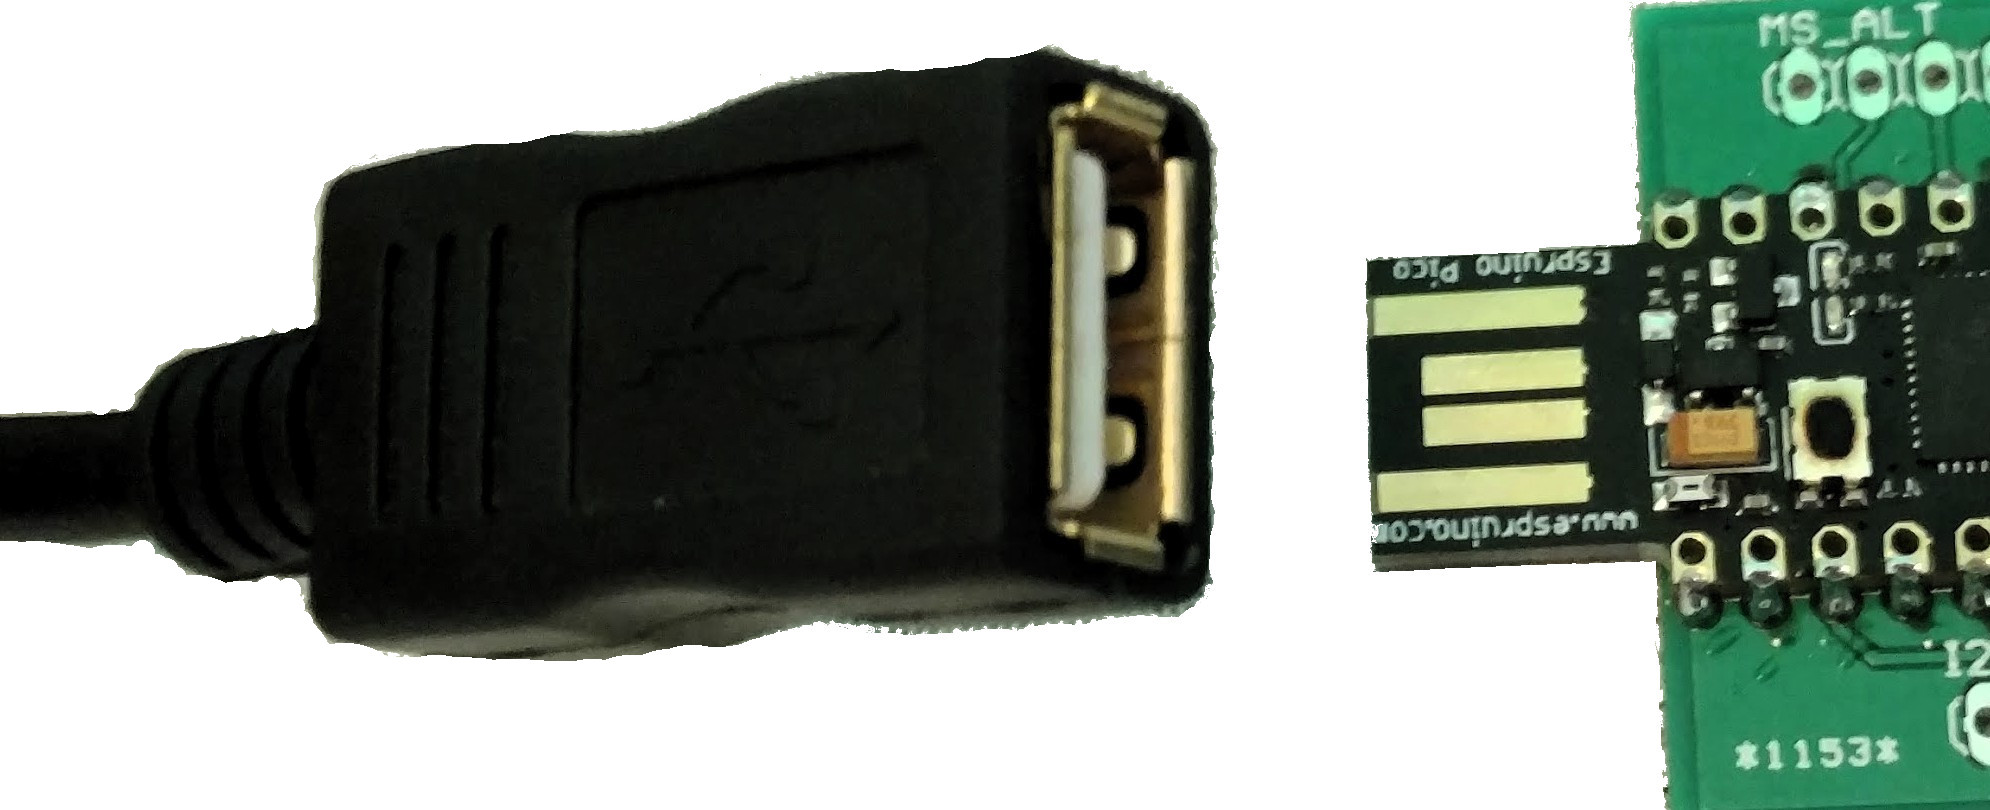
\includegraphics[width=0.5\textwidth]{images/usb.jpg}
		\caption{USB}
		\label{fig:isys}
	\end{center}
\end{figure}
	Wrong orientation can cause no damage, but the system does not work
	\item[4] Start the OpenSalinity GUI.
	\item[5] Click "Save" on the top right to chose a file to log the data too. If you want to use the default filename, just click "Open" in the file menu.
	\item[6] Start the measurement by clicking "Start".
	\item[7] Stop the measurement by clicking "Stop".
	\item[8] Repeat from step 5 for all subsequent measurements. If no new file is chosen before starting a new measurement, the data is added at the end of the previous file.
\end{itemize}